\documentclass[__main__.tex]{subfiles}

\begin{document}

\qtitle{Ч}{08}
Принципы работы лазера. Коэффициенты Эйнштейна и их взаимосвязь, распространение излучения в среде с резонансными уровнями, инверсия заселённостей, активная среда, роль резонатора.\\ 

\begin{wrapfigure}{l!}{.3\linewidth}
	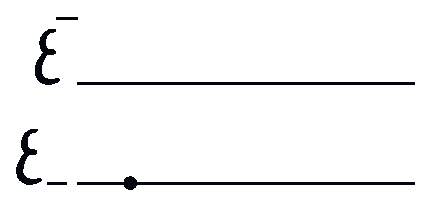
\includegraphics[scale=0.8]{ch-08-levels}
	\caption{Двухуровневая квантовая система}
	\label{ch-08-levels}
\end{wrapfigure}
Представим двухуровневую квантовую систему. На нижнем энергетическом уровне сидит электрон. Пусть в среде, "напичканной" такими квантовыми системами распространяется свет, причём энергия кванта света, фотона $\hbar\omega$ в точности равна разнице энергий верхнего и нижнего уровней. Про такую среду говорят, что она с \textbf{резонансными уровнями}:\\
$\varepsilon^{-} - \varepsilon_{-} = \hbar\omega$\\
\textbf{Вынужденное испускание фотонов}\\
Испускание фотонов, вероятность которого пропорциональна уже имеющемуся числу одинаковых фотонов, называется \textbf{вынужденным}. Так рожденные фотоны одинаково поляризованы, летят в одном направлении(так что пространственно когерентны), когерентны во времени.\\
\textbf{Спонтанное испускание}\\
Испускание фотона возможно и без наличия других фотонов, такое испускание называется \textbf{спонтанным}.\\
\textbf{Коэффициенты Эйнштейна}
Рассмотрим систему одинаковых атомов(или молекул), у которых есть пара уровней(не обязательно электронных) с энергиями $E_1$ и $E_2$, такими, что $E_2 - E_1 = \hbar\omega$.
Атом может поглотить фотон частоты $\omega$ и перейти с уровня $E_1$ и $E_2$, спонтанно испустить фотон $(E_2 \rightarrow E_1)$ и, наконец, совершить вынужденное испускание.\\
Пусть $u(\omega)$ - спектральная плотность энергии излучения на частоте $\omega$(не обязательно равновесного). Ясно, что эта величина пропорциональна числу фотонов. Обозначим $n_1$ и $n_2$ концентрации атомов с энергиями $E_1$ и $E_2$ соответственно. Тогда число переходов вверх $w\uparrow$(поглощение) и вниз $w\downarrow$(испускание) в единицу времени в единице объёма можно записать так:\\
\begin{gather}
	w\uparrow = B_{12}u(\omega)n_1,\\
	w\downarrow = An_{2} + B_{21}u(\omega)n_2
\end{gather}
$A, B$ - коэффициенты пропорциональности Эйнштейна.\\
Допустим, что речь идёт о состоянии равновесия. Тогда функция $u(w)$ есть ни что иное, как функция Планка.
\begin{gather}
	u(\omega, T) = \frac{\hbar\omega^3}{\pi^2c^3}\frac{1}{exp(\hbar\omega/kT) - 1}
	\label{ch-08-plank}
\end{gather}
В силу принципа детального равновесия должно быть $w\uparrow = w\downarrow$, т.е.
\begin{gather}
	B_{12}u(\omega, T)n_1 = An_2 + B_{21}u(\omega, T)n_2
	\label{ch-08-4}
\end{gather}
Сначала перейдём к пределу $T\rightarrow \infty$. В этом пределе $u(\omega, T) \rightarrow \infty$, так что членом $An_2$ можно пренебречь, кроме того, $\frac{n_2}{n_1} =e^{-\frac{\hbar\omega}{kT}} \rightarrow 1.$ Таким образом, $B_{12} = B_{21} = B$. Теперь вернёмся к соотношению \ref{ch-08-4}, разделим обе части на $n_2$ и перенесём члены, содержащие $u(w, T)$ влево:
$$Bu(\omega, T)(e^{\frac{\hbar\omega}{kT}} - 1) = A$$ 
Подставляя функцию Планка \ref{ch-08-plank}, получаем
$$
A = \frac{\hbar\omega^3}{\pi^2c^3}B
$$
\begin{definition}[Инверсия населённостей]
	\textbf{Инверсией населённостей} называется неравновесное состояние вещества, при котором $n_2 > n_1$, а среда с инверсией \textbf{активной средой}.  
\end{definition}
\textbf{Работа лазера}

\begin{wrapfigure}{l!}{.3\linewidth}
	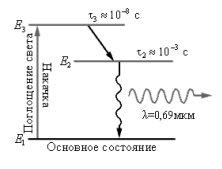
\includegraphics{ch-08-triple}
	\caption{Трёхуровневая схема лазерного усилителя светового потока.}
	\label{ch-08-triple}
\end{wrapfigure}
Представленные параметры характерны для классического лазера на рубине, с той лишь разницей, что верхний уровень $E_3$ в рубине представляет собой две широкие энергетические зоны. Это важно потому что для перевода электронов с основного уровня на верхний (накачка) можно использовать лампы с довольно широким спектром.\\
С этого верхнего уровня(среднее время жизни на нём $~10^{-8}$с) электроны безызлучательно переходят на метастабильный уровень $E_2$, где могут жить гораздо дольше ($~10^{-3}$с), потому что там и накапливаются. Рабочие уровни - уровни $E_1$ и $E_2$, именно на них образуется инверсия населённостей. Если после накачки через кристалл пропустить свет с длиной волны, соответствующей переходу между этими уровнями энергии, то его интенсивность будет усиливаться за счёт преобладания вынужденного испускания над поглощением.\\
Это пока когерентный усилитель света. Чтобы получился лазер, его надо преобразовать в генератор. Эта задача всегда решается одинаково, включением положительной обратной связи, которую обеспечивают устройства, называющиеся \textbf{открытыми резонаторами}.
В простейшем случае они представляют собой два плоских параллельных зеркала, между которыми помещается кристаллический стержень с осью, перпендикулярной к поверхности зеркал. Одно из зеркал должно быть полупрозрачным для вывода излучения наружу. В общем случае устройство оптического резонатор может быть более сложным. Резонаторы не только обеспечивают возможность генерации света в лазере, но и могут улучшать его пространтсвенную (сохраняя только лучи, параллельные оси) и  временную(вырезая из широкой атомной линии более узкую спектральную часть) когерентность.\\
Процесс генерации начинается со спонтанного рождения удачных фотонов, летящих вдоль оси резонатора. Отражаясь от зеркал и вновь проходя через активную среду, они вызыва.т вынужденное излучение, также многократно отражающееся от зеркал. Это лавинный процесс. Рост плотности энергии излучения приводит к росту числа вынужденных переходов - к росту плотности излучения. Этот процесс продолжается до тех пор, пока неизбежные потери не превысят скорость генерации новых фотонов.
\end{document}